% !TeX spellcheck = <none>
\documentclass{report}
\usepackage{graphicx}
\usepackage[portuguese]{babel}
\usepackage[utf8]{inputenc}
\usepackage{hyperref}
\usepackage{indentfirst}
%\usepackage[latin1]{inputenc}
%\usepackage{url}
\usepackage{color}
\usepackage{enumerate}
\usepackage{alltt}
\usepackage{fancyvrb}
\usepackage{listings}
\usepackage{amsmath}
\newcommand{\keyword}[1]{\textsf{#1}}

\DefineVerbatimEnvironment{code}{Verbatim}{fontsize=\footnotesize}
%LISTING - GENERAL
\lstset{
	basicstyle=\small,
	numbers=left,
	numberstyle=\tiny,
	numbersep=5pt,
	breaklines=true,
    frame=tB,
	mathescape=true,
	escapeinside={(*@}{@*)}
	}


\title{Processamento de Linguagens e Compiladores\\ (3º ano de LCC)\\ \textbf{Galo}\\ TP3\\ Grupo 14}
\author{Artur Queiroz\\ A77136 \and  Rafael Fernandes\\ A78242 \and Rafaela Pinho\\ A77293 }
\date{\today}

\begin{document}
	
\maketitle
	

\begin{abstract}
	Neste relatório apresentamos a linguagem que criamos e o complidor que gera o código para a Máquina Virtual VM.
\end{abstract}

\tableofcontents

\chapter{Introdução} \label{intro}
\indent
Neste relatório apresentamos o último trabalho da unidade curricular "Processamento de Linguagens e Compliadores". Este consiste em desenvolver um processador de linguagens usando o método da tradução dirigida pela sintaxe. Também devemos desenvolver um compilador que gera o código para uma máquina de stack virtual. Utilizaremos a ferramenta Yacc para gerar compiladores baseados em gramáticas tradutoras.\\
\indent
Como todos os outros trabalhos, este também tem como objetivo aumentar a experência no uso do ambiente Linux, da linguagem C e  ferramentas de apoio à programção.\\
\indent
Este relatório está dividido em 4 partes. No primeiro capítulo encontramos a parte introdutório a este trabalho, onde explicamos no que consiste. No capítulo 2 (dois) apresentamos os requisitos e a linguagem que criamos. No terceiro mostramos as decisões e alguns teste efectuados. No último temos a conclusão e os objetivos do trabalho futuro.
 
\chapter{Galo e Compilador} \label{fi}
\section{Descrição informal do problema}
\indent
Neste trabalho foi pedido para criarmos uma linguagem de programação imperativa e desenvolver um compilador para a linguagem criada.\\
\indent
Na linguagem as declarações de variáveis devem ser colocadas no início do programa, não pode haver re-declarações e não se pode usar variáveis sem estar declaradas primeiro. Caso não seja atribuido uma valor à variável depois da declaração, esta ficará com o valor zero.\\
\indent  	
O complilador deve gerar o código assembly para a Máquina Virtual VM.

\section{Especificação dos requisitos}
\indent
Para este tarbalho a linguagem que criamos tem de conter os seguintes requisitos:
\begin{enumerate}
	\item Declarar e manusear variáveis atómicas do tipo inteiro e estruturas do tipo array de inteiros.
	\item Ler do standard input e escrever no standard output.
	\item Fazer instruções básicas como a atribuição de expressões a variáveis.
	\item definir e invocar subprogramas sem parâmetros mas que possam retornar um resultado atómico.
	\item efetuar instruções para controlo do fluxo de execução—condicional e cíclica—que possam ser aninhadas.
\end{enumerate}
\indent
Também devrá conter um conjunto de testes (escritos na nossa linguagem) que tem de ter no mínino os 6 exemplos seguintes:
\begin{enumerate}[i)]
	\item Ler 4 números e dizer se podem ser os lados de um quadrado.
	\item Ler um inteiro N, depois ler N números e escrever o menor deles.
	\item Ler N (constante do programa) números e calcular e imprimir o seu produtório.
	\item Contar e imprimir os números impares de uma sequência de números naturais.
	\item Ler e armazenar os elementos de um vetor de comprimento N; imprimir os valores por ordem decrescente após
	fazer a ordenação do array por trocas diretas.
	\item Ler e armazenar N números num array; imprimir os valores por ordem inversa
\end{enumerate} 
\section{Expressões regulares} 
As expressões regulares usadas foram:

\begin{enumerate}
	\item \#.*\$  
	\item $\backslash$"[\^\"]* $\backslash$"
	\item $[ ]+e[ ]+$
	\item $[ ]+ou[ ]+$
	\item $[ ]+sin[ ]+$
	\item $[ ]+cos[ ]+$
	\item ==
	\item $\backslash$$<=$
	\item $\backslash$$>=$
	\item !=
	\item $[$=;\{\}(),$<>$!$\backslash$+$\backslash$-$\backslash$*$\backslash$/\%$\backslash$[$\backslash$]]
	\item se$|$SE
	\item senao$|$SENAO 
	\item caso$|$CASO
	\item enq$|$ENQ
	\item return
	\item $[$0-9]+$\backslash$.[0-9]+ 
	\item int$|$string$|$float 
	\item$[$0-9]+
	\item $[$a-zA-Z][a-zA-Z0-9]*
	\item $[$$\backslash$t$\backslash$n] 
	
\end{enumerate}

\section{A nossa linguagem}
\subsection{Galo}
\indent
Como já referido em cima, foi-nos pedidos para criar uma linguagem de programação. Decidimos chamar de Galo por ser um símbolo típico de Potugal, e atribuimos .gl para a extensão.\\
\indent
Para a definirmos utilizamos uma gramática independente do contexto, em que tomamos certas decisões que serão especificadas.\\
\indent
O Galo reconhece os segintes tipos: números inteiros (int), números décimais  (float) e conjunto de caractéres (string). A linguagem usa os habituais síbolos de comparação, como $<=$, $>=$, $==$ e $!=$. Utiliza o "e" e o "ou" como símbolos de operadores lógicos.\\
\indent
Como a nossa linguagem é muito parecida ao C, para fazer o "ite" utilizamos o "se" e o "senao" (tanto minúsculo como maiúsculo) para o "while" usamos o "enq" ou "ENQ".\\
\indent
Existe as funções "ler?()" e "escrever?()" que são, respetivamente, a função de leitura no teclado e de escrita no ecrã. (? = i ou s ou f, i-inteiro, s-string, f- float) \\

\indent
A nossa linguagem está definida pela seguinte GIC:

\begin{code}
	
	1 ProgG: ProgG Se
	2      | ProgG Enq
	3      | ProgG Atrib ';'
	4      | ProgG VAR '=' Expr ';'
	5      | ProgG VAR '[' Expr ']' '=' Expr ';'
	6      | ProgG CriaFun
	7      | ProgG Funcao ';'
	8      | ProgG ';'
	9      | ProgG COM
	10     | %empty
	
	11 ProgF: ProgF Se
	12      | ProgF Enq
	13      | ProgF Atrib ';'
	14      | ProgF VAR '=' Expr ';'
	15      | ProgF VAR '[' Expr ']' '=' Expr ';'
	16      | ProgF Funcao ';'
	17      | ProgF ';'
	18      | ProgF COM
	19      | ProgF RETURN Expr ';'
	20      | %empty
	
	21 Prog: Prog Se
	22     | Prog Enq
	23     | Prog Atrib ';'
	24     | Prog VAR '=' Expr ';'
	25     | Prog VAR '[' Expr ']' '=' Expr ';'
	26     | Prog Funcao ';'
	27     | Prog ';'
	28     | Prog COM
	29     | %empty
	
	30 Funcao: VAR Lexpr
	
	31 CriaFun: TIPO VAR '('
	32        | Ltipo '{' ProgF '}'
	
	33 Atrib: TIPO VAR
	34      | TIPO VAR '[' Expr ']'
	35      | Igual
	
	36 Igual: TIPO VAR '='
	37      | TIPO VAR '[' Expr ']' '='
	38      | Igual Expr
	
	39 Lexpr: '(' ')'
	40      | '(' Eexpr ')'
	
	41 Eexpr: Expr
	42      | Eexpr ',' Expr
	
	43 Ltipo: ')'
	44      | Etipo ')'
	
	45 Etipo: TIPO VAR
	46      | Etipo ',' TIPO VAR
	
	47 Se: SE Cond
	48   | Se '{' Prog '}' SENAO
	49   | Se '{' Prog '}'
	
	50 Enq: ENQ
	51    | Enq Cond
	52    | Enq '{' Prog '}'
	
	53 Cond: NUM
	54     | '(' Expr EQ Expr ')'
	55     | '(' Expr NEQ Expr ')'
	56     | '(' Expr '<' Expr ')'
	57     | '(' Expr '>' Expr ')'
	58     | '(' Expr LEQ Expr ')'
	59     | '(' Expr GEQ Expr ')'
	60     | '(' Cond E Cond ')'
	61     | '(' Cond OU Cond ')'
	62     | '!' Cond
	
	63 Sexpr: VAR
	64      | NUM
	65      | FLOAT
	66      | VAR '[' Expr ']'
	67      | Funcao
	68      | STR
	
	69 Expr: '(' Expr '+' Expr ')'
	70     | '(' Expr '-' Expr ')'
	71     | '(' Expr '*' Expr ')'
	72     | '(' Expr '/' Expr ')'
	73     | '(' Expr '%' Expr ')'
	74     | COS Expr
	75     | SIN Expr
	76     | '(' Expr ')'
	77     | Sexpr
	
\end{code}

\chapter{Codificação e Testes}
\section{Problemas de implementação, Decisões e Alternativas}
\subsection{Problemas de implementação}
\indent
Como em todos os trabalhos tivemos alguns contratempos, dos quais muitos foram superados.\\
\indent
Quando estavamos a passar a nossa linguagem para uma gramática tradutora tivemos alguns prblemas com o código assembly da máquina virtual, mas nada que não se resolvesse com um bocadinho de paciência e trabalho de grupo. Tivemos também problemas na implementação de vetores.   
   


\subsection{Decisões}
\begin{enumerate}[1)]
	\item O "e" ($\&\&$) está definida pela multuplicação e o "ou" ($||$) pela adição.
 
	 \begin{table}[h]
		\begin{center}
	 	\caption{Tabela do E}
	 	\begin{tabular}{r|lr}
	 	 *(E)& 0 & 1\\ % Note a separação de col. e a quebra de linhas
	 	\hline          % para uma linha horizontal
	 	0 & 0 & 0 \\
	 	1 & 0 & 1\\
 	
		\end{tabular}
		\caption{Tabela do OU}
		\begin{tabular}{r|lr}
		+(OU)& 0 & 1\\ % Note a separação de col. e a quebra de linhas
		\hline          % para uma linha horizontal
		0 & 0 & 1 \\
		1 & 1 & 2\\
		\end{tabular}
		\end{center}
	\end{table}

	\item Não se pode declarar mais do que uma variável numa linha, ou seja todas as declarações são individuais.\\
	 Exemplo: \\int a = 2 , c = 0;\\ terá de ser:\\
	 int a = 2;\\
	 int c = 0;\\
	 \item Não se pode fazer "return" dentro dos Se's e dos Enq's.\\ 
	 \item Nas expressões numéricas, as operações binárias têm de estar sempre dentro de parênteses.\\
	 Exemplo:\\
	 int a = (1+(2*3))
	 \item todo o codigo dentro de se's, enq's e funções começa em $\{$ e acaba em  $\}$.
	 
	
\end{enumerate}

\section{Testes realizados e Resultados}
\subsection{Exemplos escritos na nossa linguagem}

\begin{enumerate}
	\item Ler 4 números e dizer se podem ser os lados de um quadrado.\\
	
	\begin{code}
	int a = leri();
	int b = leri();
	int c = leri();
	int d = leri();
	
	se ((a==b) e ((b==c) e (c==d))) {
		escrevers("É um quadrado\n");
	}
	senao {
		escrevers("Não é um quadrado\n");
	}
	\end{code}	
	
	\item Ler um inteiro N, depois ler N números e escrever o menor deles.\\
	
	\begin{code}
		escrevers("Escreva o número de elementos do array:\n");
		int N = leri();
		
		int i = 0;
		int a = 0;
		int res = 0;
		
		se (N!=0){
			res = leri();
			i = 1;
			enq (i < N){
				a = leri();
				
				se (res > a){
					res = a;
				}
				
				i = (i+1);
			}
			
			
			escrevers("O menor número foi o ");
			escreveri(res);
			escrevers("\n");
			
		}
		senao{
			escrevers("Não leu nenhum número\n");
		}
	\end{code}
	
	\item Ler N (constante do programa) números e calcular e imprimir o seu produtório.\\
	
	\begin{code}
		escrevers("Vão se ler 5 números\n");
		
		int N = 5;
		int i = 0;
		int r = 1;
		
		enq(i < N){
			
			r = (r * leri());
			
			i = (i + 1);
		}
				
		escrevers("O produtório desta sequencia de 5 números é ");
		escreveri(r);
		escrevers("\n");
	\end{code}

	\item Contar e imprimir os números impares de uma sequência de números naturais.\\
	
	\begin{code}
		escrevers("Digitar uma sequência de números, termina quando for zero\n");
		
		int cont = 0;
		int i = leri();
		
		enq(i != 0){
			se ((i % 2) == 1){
				cont = (cont + 1);
				escreveri(i);
				escrevers(" \n");
			}
			i = leri();
		}
	
	escrevers("Foram lidos ");
	escreveri(cont);
	escrevers(" impares \n");
	\end{code}
 
  	\item Ler e armazenar os elementos de um vetor de comprimento N; imprimir os valores por ordem decrescente após
	fazer a ordenação do array por trocas diretas.\\
	
	\begin{code}
		int troca(int v, int i, int j){
			int k = v[i];
			v[i] = v[j];
			v[j] = k;
			return 0;
		}
		
		int ordena(int* v, int N){
			int i = 0; #inicio
			int j = 0; #procura
			int m ;    #pos do menor
			
			enq (i<(N-1)){
				j = (i + 1);
				m = i;
				enq (j<N){
					se(v[j]>v[m]){
						m = j;
					}
					j = (j + 1);
				}
				troca(v,i,m);
				i = (i + 1);
			}
			return 0;
		}
		
		int N = leri();
		int i = 0;
		int v[N];
		
		enq(i<N){
			v[i] = leri();
			i = (i+1);
		}
		
		ordena(v, N);
		
		i = 0;
		
		enq(i<N){
			escreveri(v[i]);
			escrevers("\n");
		}
	\end{code}	
	
	\item Ler e armazenar N números num array; imprimir os valores por ordem inversa.\\
	
	\begin{code}
		int N = leri();
		int i = 0;
		int a = 0;
		int v[N];
		
		enq (i < N){
			v[i] = leri();
			i = (i + 1);
		}
		
		enq(i > 0){
			a = v[(i-1)];
			escreveri(a);
			escrevers("\n");
			i = (i-1);
		}
	\end{code}

\end{enumerate}

\subsection{Resultados}
\indent
Depois de executarmos os comados seguintes:\\
\noindent
\$ flex -o galo.c galo.l\\
\$ yacc -d -v galo.y\\
\$ gcc -o galo y.tab.c -lm\\
compilamos todos os nossos exemplos.\\
\indent
Obtivemos o seguinte resultado:
\begin{enumerate}
	\item Ler 4 números e dizer se podem ser os lados de um quadrado.
	\begin{code}
		
	start
	pushi 0
	read
	atoi
	storeg 0
	pushi 0
	read
	atoi
	storeg 1
	pushi 0
	read
	atoi
	storeg 2
	pushi 0
	read
	atoi
	storeg 3
	pushg 0
	pushg 1
	equal
	pushg 1
	pushg 2
	equal
	pushg 2
	pushg 3
	equal
	mul
	mul
	jz fimse0
	pushs "É um quadrado\n"
	writes
	jump fimse1
	fimse0:
	pushs "Não é um quadrado\n"
	writes
	fimse1:
	stop
	
	\end{code}
	\indent
	Após abrir o ficheiro na máquina virtual, se atribuirmos, por exemplo, o número 4 ao a, b, c, d o programa retorna \textbf{"É um quadrado"} (Figura A.1). Se atribuinos valores diferentes ao a, b, c, d o programa diz \textbf{"Não é um quadrado"} (Figura A.2).
	
	
	\item Ler um inteiro N, depois ler N números e escrever o menor deles.
	
	\begin{code}
		start
		pushs "Escreva o número de elementos do array:\n"
		writes
		pushi 0
		read
		atoi
		storeg 0
		pushi 0
		pushi 0
		storeg 1
		pushi 0
		pushi 0
		storeg 2
		pushi 0
		pushi 0
		storeg 3
		pushg 0
		pushi 0
		equal
		pushi 0
		equal
		jz fimse0
		read
		atoi
		storeg 3
		pushi 1
		storeg 1
		enq0:
		pushg 1
		pushg 0
		inf
		jz fimenq0
		read
		atoi
		storeg 2
		pushg 3
		pushg 2
		sup
		jz fimse1
		pushg 2
		storeg 3
		fimse1:
		pushg 1
		pushi 1
		add
		storeg 1
		jump enq0
		fimenq0:
		pushs "O menor número foi o "
		writes
		pushg 3
		writei
		pushs "\n"
		writes
		jump fimse2
		fimse0:
		pushs "Não leu nenhum número\n"
		writes
		fimse2:
		stop
		
	\end{code}

	\indent
	Defininos que o array tem 3 elementos e depois digitamos valores, por exemplo o 7, 5 e o 8. O resultado deste programa é o menor desses elementos, que é o 5 (figura A.3). Se o array tivesse 0 elementos o programa diz que " 
	Não leu nenhum número" (figura A.4).
	\item Ler N (constante do programa) números e calcular e imprimir o seu produtório.
	
	\begin{code}
		start
		pushs "Vão se ler 5 números\n"
		writes
		pushi 0
		pushi 5
		storeg 0
		pushi 0
		pushi 0
		storeg 1
		pushi 0
		pushi 1
		storeg 2
		enq0:
		pushg 1
		pushg 0
		inf
		jz fimenq0
		pushg 2
		read
		atoi
		mul
		storeg 2
		pushg 1
		pushi 1
		add
		storeg 1
		jump enq0
		fimenq0:
		pushs "O produtório desta sequencia de 5 números é "
		writes
		pushg 2
		writei
		pushs "\n"
		writes
		stop
		
	\end{code}

	\indent
	Atribuimos 5 como o numero de elementos do array. de pois digitamos a sequência 3,4,5,6,8 de e o resultado do programa de 2880 que é o produtório da sequência (figura A.5).	
	
	\item Contar e imprimir os números impares de uma sequência de números naturais.
	
	\begin{code}
		start
		pushs "Digitar uma sequência de números, termina quando for zero\n"
		writes
		pushi 0
		pushi 0
		storeg 0
		pushi 0
		read
		atoi
		storeg 1
		enq0:
		pushg 1
		pushi 0
		equal
		pushi 0
		equal
		jz fimenq0
		pushg 1
		pushi 2
		mod
		pushi 1
		equal
		jz fimse0
		pushg 0
		pushi 1
		add
		storeg 0
		pushg 1
		writei
		pushs " \n"
		writes
		fimse0:
		read
		atoi
		storeg 1
		jump enq0
		fimenq0:
		pushs "Foram lidos "
		writes
		pushg 0
		writei
		pushs " impares \n"
		writes
		stop
		
	\end{code}
	
	\indent
	Começa por aparecer a mensagem para digitarmos uma sequência de números. 
	Digitando os valores 3, 1, 2, 6, 5 e 0. À medida que vamos inserindo os números vão aparecendo os que são impares. Depois quando digitamos o zero aprece a quantidade de números impares que foram lidos. (figura A.6).
	
	\item Ler e armazenar os elementos de um vetor de comprimento N; imprimir os valores por ordem decrescente após
	fazer a ordenação do array por trocas diretas.
	
	\begin{code}
		
	\end{code}

	\indent
	
	
	\item Ler e armazenar N números num array; imprimir os valores por ordem inversa.
	
	\begin{code}
		
		atoi
		storeg 0
		pushi 0
		pushi 0
		storeg 1
		pushi 0
		pushi 0
		storeg 2
		pushg 0
		storeg 3
		enq0:
		pushg 1
		pushg 0
		inf
		jz fimenq0
		pushg 1
		read
		atoi
		pushg 1
		pushi 1
		add
		storeg 1
		jump enq0
		fimenq0:
		enq1:
		pushg 1
		pushi 0
		sup
		jz fimenq1
		pushg 1
		pushi 1
		sub
		storeg 2
		pushg 2
		writei
		pushs "\n"
		writes
		pushg 1
		pushi 1
		sub
		storeg 1
		jump enq1
		fimenq1:
		stop
		
	\end{code}

	\indent
	
	
\end{enumerate}
  





\chapter{Conclusão} \label{concl}
 \indent
 Este trabalho abrangeu maior parte da matéria lecionada ao longo do semestre. Através do nosso conhecimento em GIC's e sobre o gerador Yacc e Flex criamos um compilador para converter a nossa linguagem em código assembly para a Máquina Virtual VM.\\
 Não coseguimos acabar todas as tarefas propostas, o exemplo 5 e 6 não estão a funcionar devido aos vetores. Como referido no capítulo 3 tivemos dificuldades a implementar essa estrutura.\\
 \indent
 Como trabalho futuro gostaríamos de implementar os vetores e adicionar mais elementos à nossa linguagem. 

\appendix
\chapter{Imagens}

\begin{figure}[h]
	\centering
	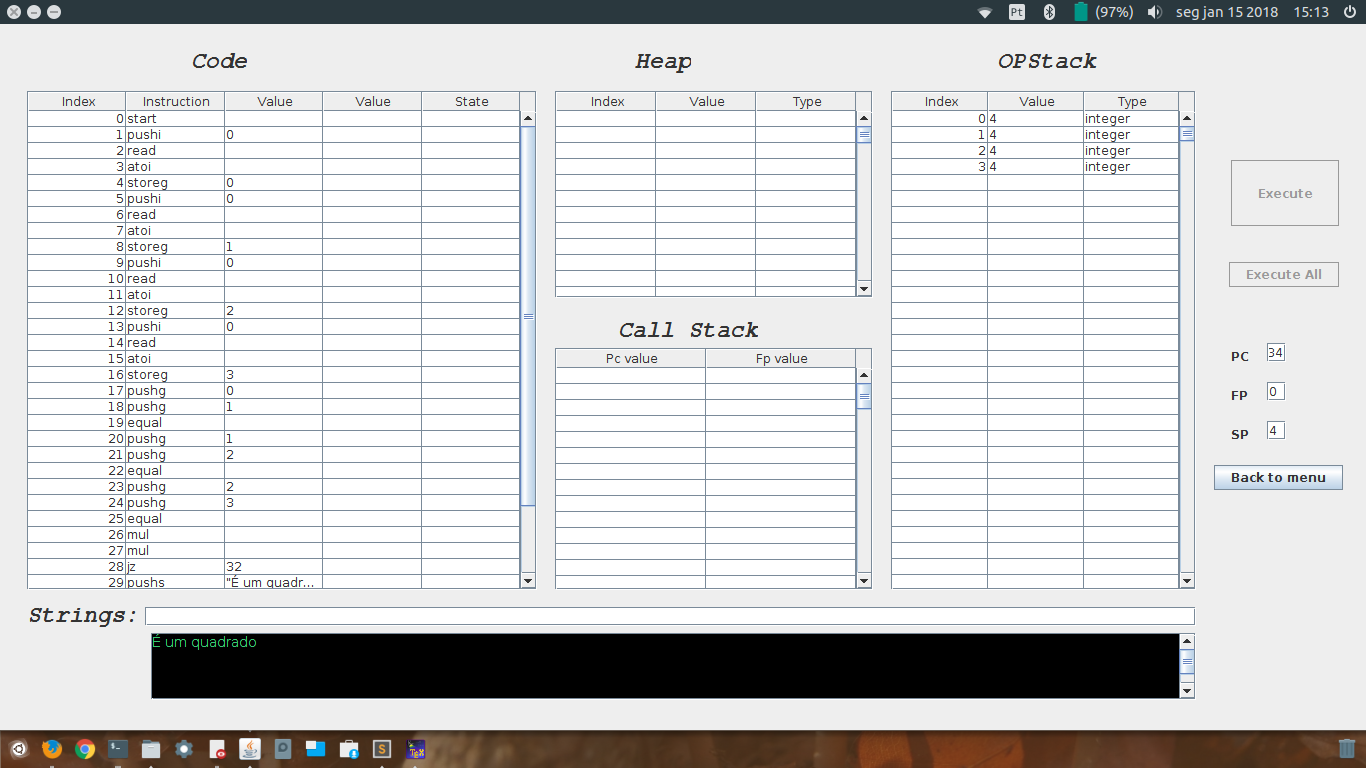
\includegraphics[width=9cm,height= 5cm]{exemplo1-1.png}
	\caption{Verifica se é um quadrado}
	\label{Exemplo 1.1}
\end{figure}

\begin{figure}[h]
	\centering
	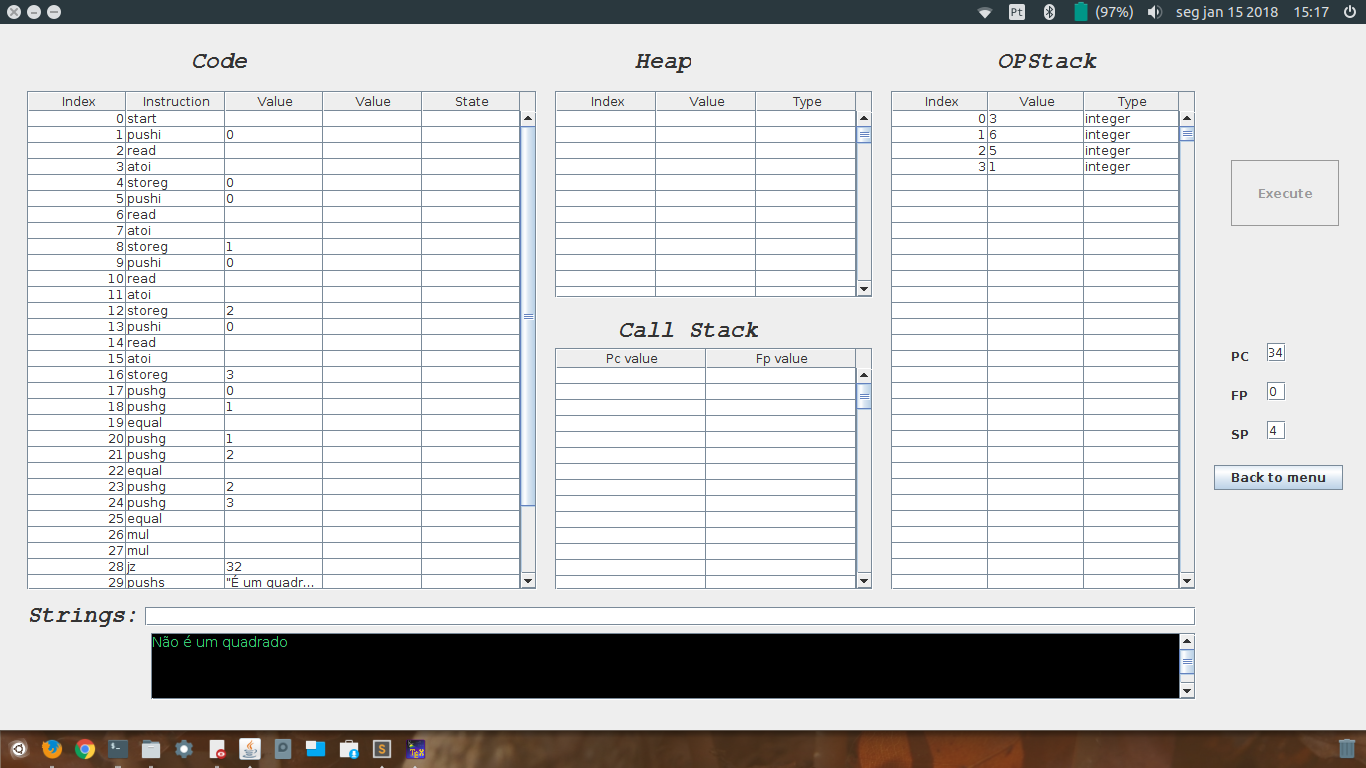
\includegraphics[width=9cm,height= 5cm]{exemplo1-2.png}
	\caption{Verifica que não é um quadrado}
	\label{Exemplo 1.2}
\end{figure}

\begin{figure}[h]
	\centering
	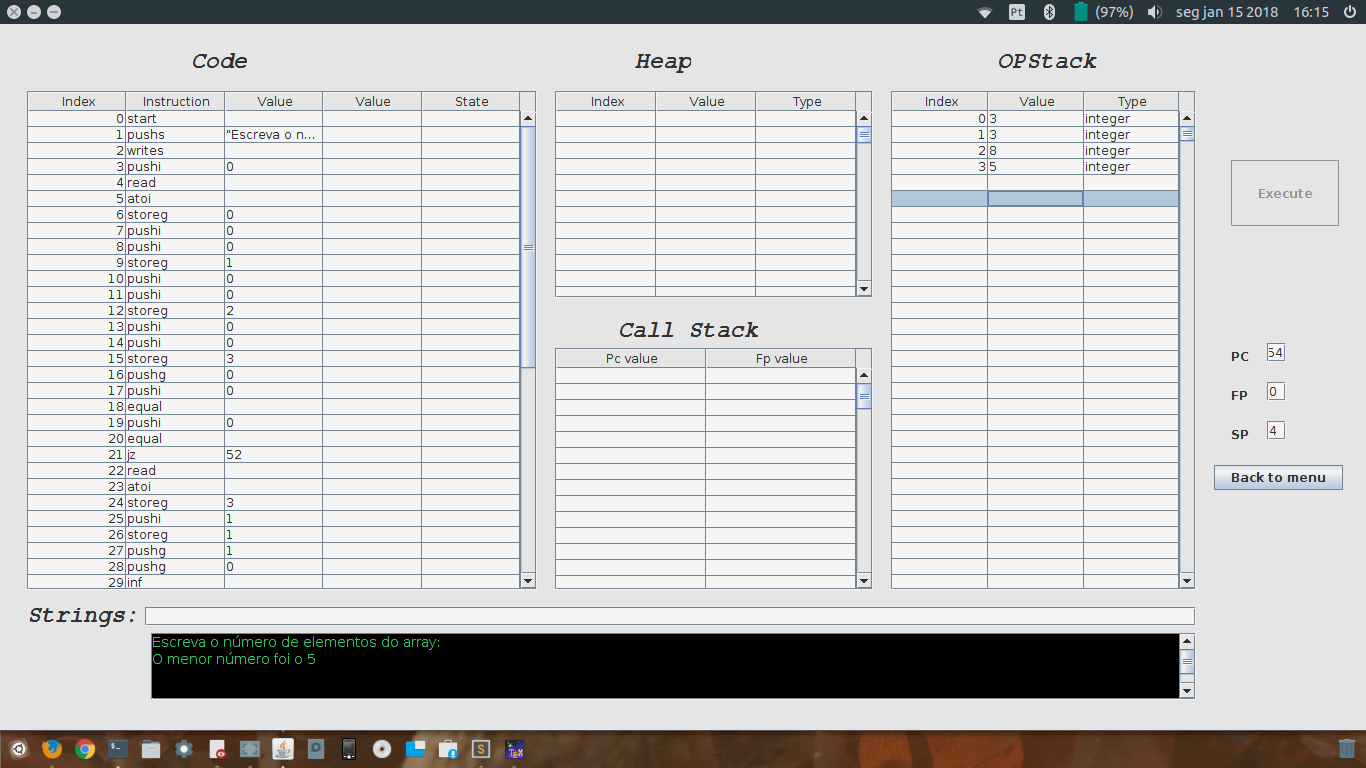
\includegraphics[width=9cm,height= 5cm]{exemplo2-1.png}
	\caption{Diz qual é o menor número}
	\label{Exemplo 2.1}
\end{figure}

\begin{figure}[h]
	\centering
	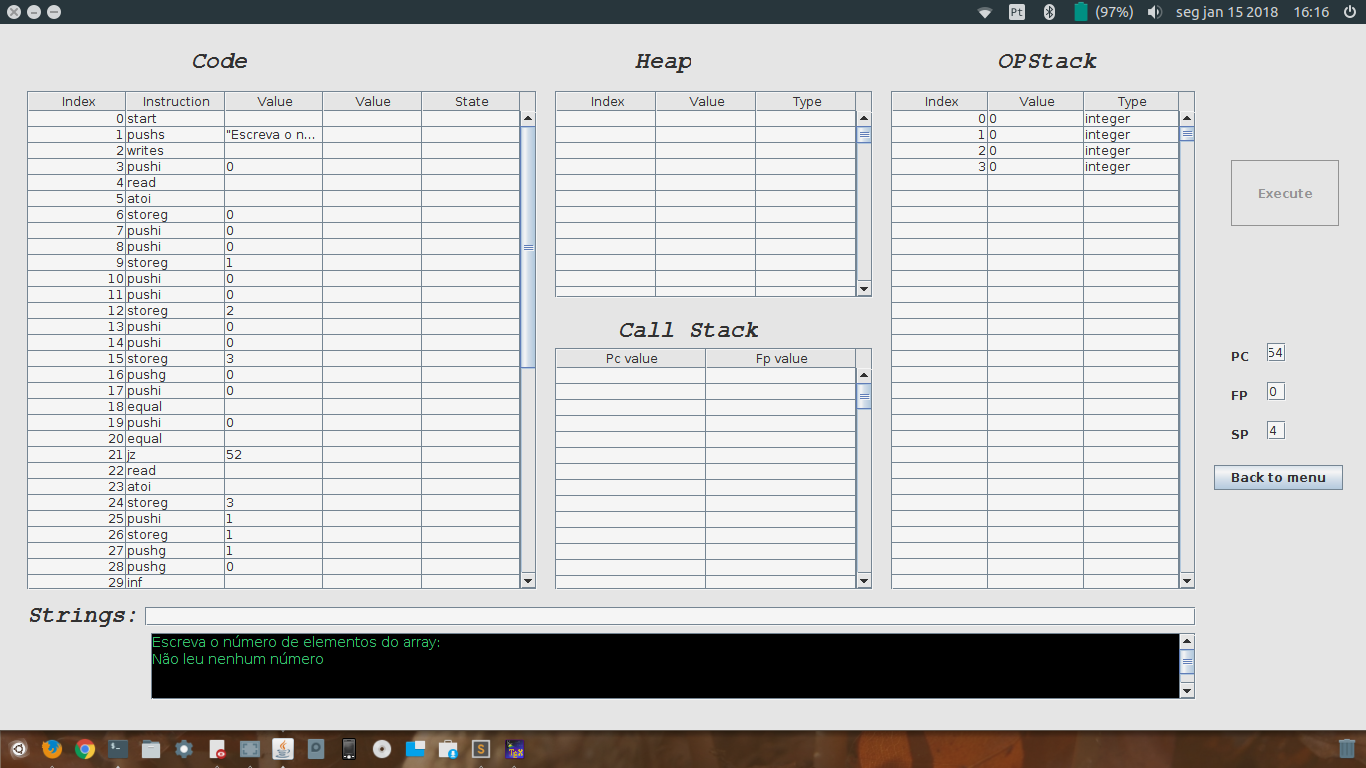
\includegraphics[width=9cm,height= 5cm]{exemplo2-2.png}
	\caption{Verifica que não leu nenhum número}
	\label{Exemplo 2.2}
\end{figure}

\begin{figure}[h]
	\centering
	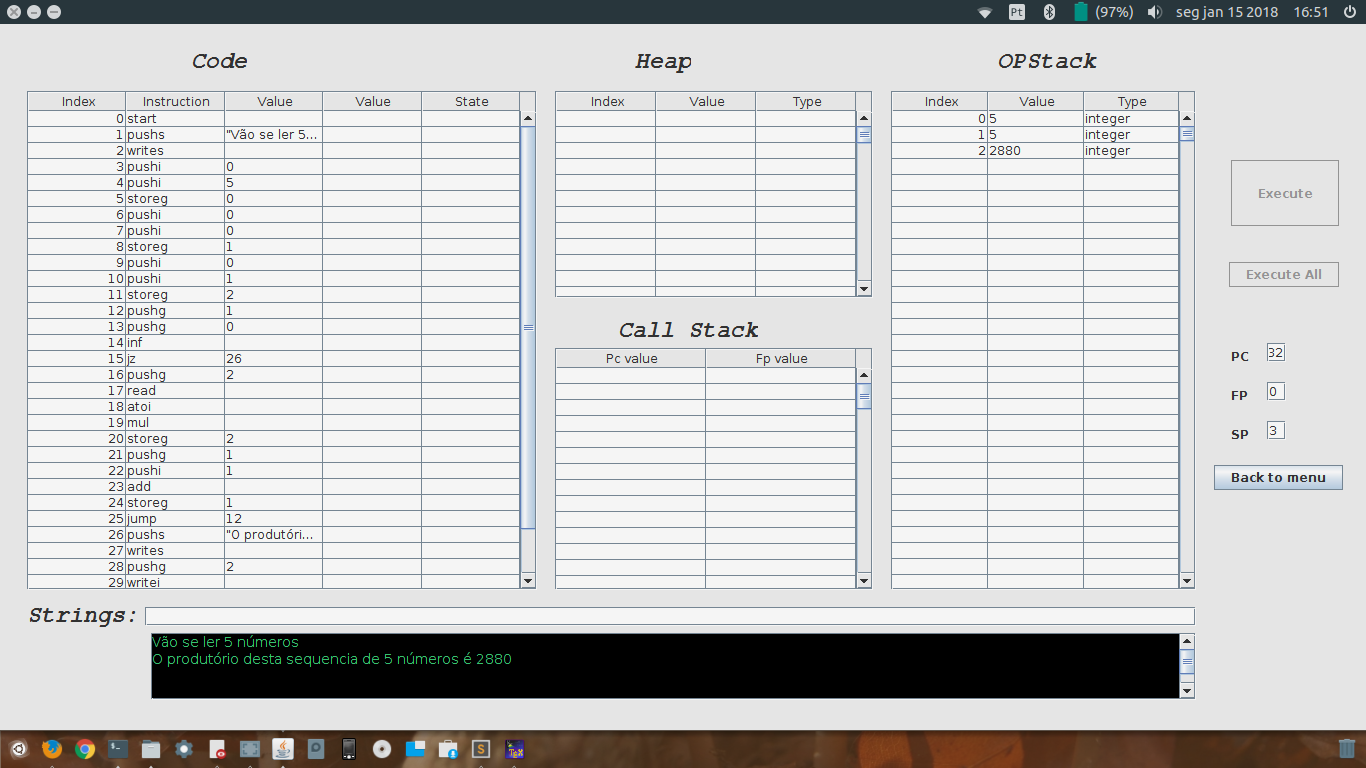
\includegraphics[width=9cm,height= 5cm]{exemplo3-1.png}
	\caption{Apresenta o produtório}
	\label{Exemplo 3.1}
\end{figure}

\begin{figure}[h]
	\centering
	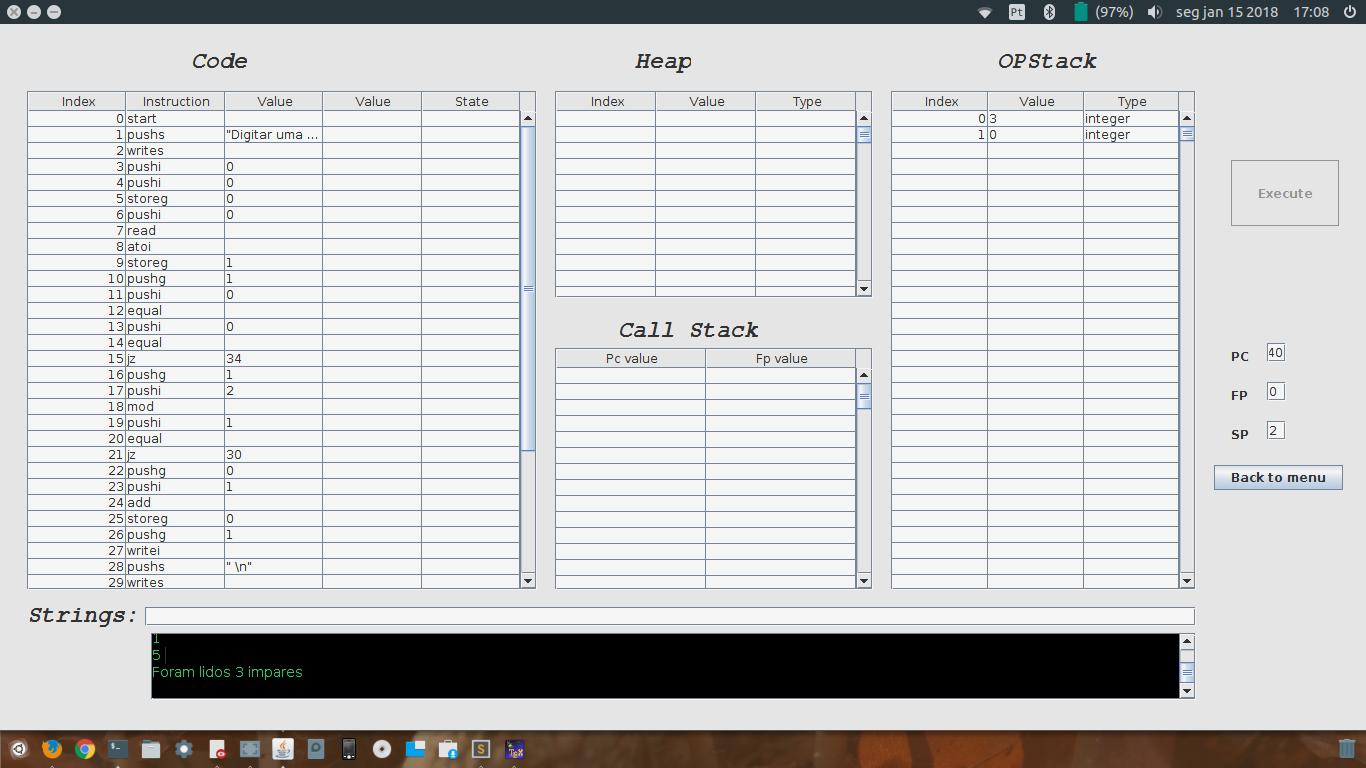
\includegraphics[width=9cm,height= 5cm]{exemplo4-1.png}
	\caption{Mostra quantos impares foram lidos}
	\label{Exemplo 4.1}
\end{figure}








\end{document}